In many situations, functional observations have
similar shapes, but they are in some way misaligned. This variability can
interfere with further analysis. Therefore, it is desirable quantify and
eliminate or reduced this variation. This process is called \textit{registration}.


\begin{figure}[Male growth rate]{FIG:BERKELEY}{Male growth rate}
	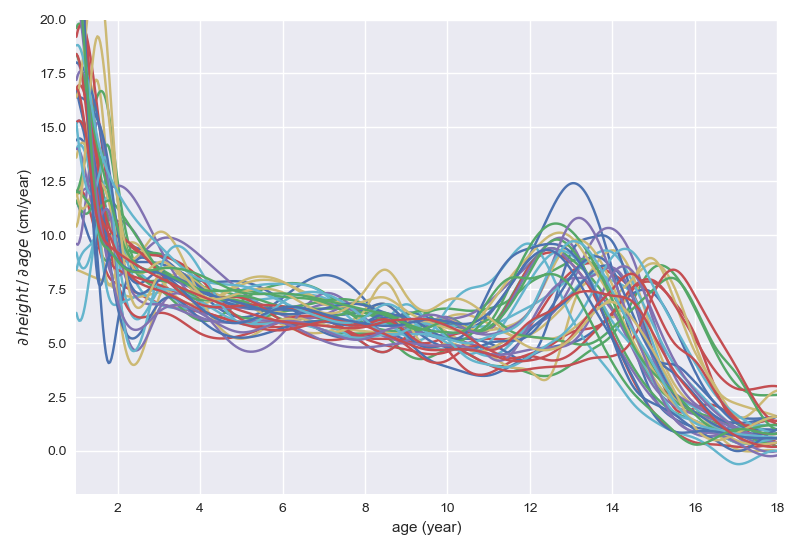
\includegraphics[width=11cm]{berkeley-males}
\end{figure}

To illustrate the problem we consider functional data from the Berkeley Growth
Study\cite{berkeley}. In this 1954 study, the heights of 54
girls and 39 boys between the ages of 1 and 18 years were recorded. In Figure
\ref{FIG:BERKELEY} velocity growth curves of the boys are shown.
These curves correspond to the derivatives of the growth curves. In them this
type of variability may be appreciated in a more pronounced way.
Every curve shows a main stage of growth corresponding with the puberty;
however, these stages are not aligned due to hormonal and other
physiological factors in the growth. The rigid metric of physical time may not
be directly relevant to the internal dynamics of our problem. Thus it may be
convenient to make a transformation of the time scale to adapt it to the nature
of our data. In the registration of the data, or alignment, this type of
variability is analyzed, quantified and separated.

%\cite{Kokoszka2017}

The variability of the data can be analyzed in terms of amplitude and
phase variation. \textit{Amplitude variation} corresponds to the
random curve-to-curve variation.
In the Figure \ref{SBFIG:AMPLITUDE} a
set of curves whose variability proceeds exclusively from the amplitude is shown.
\textit{Phase variation} refers to
misalignments of the curves with respect to the
domain. In the Figure
\ref{SBFIG:PHASE} a set of curves whose variation is completely due
to the phase is shown; this source of variability is the one that will be dealt with in
the registration process.

\begin{figure}[Amplitude and phase variability]{FIG:AMPPHA}{Amplitude and phase variability}
  \subfigure[SBFIG:AMPLITUDE]{Dataset with amplitude variability}{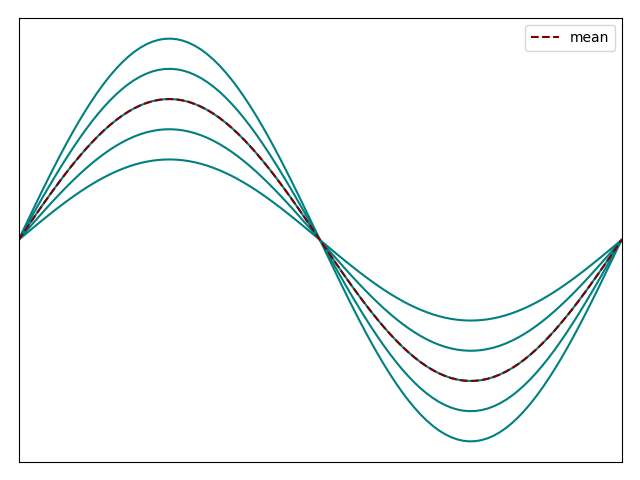
\includegraphics[width=7.5cm]{amplitude-variation}} \quad
  \subfigure[SBFIG:PHASE]{Dataset with phase variability}{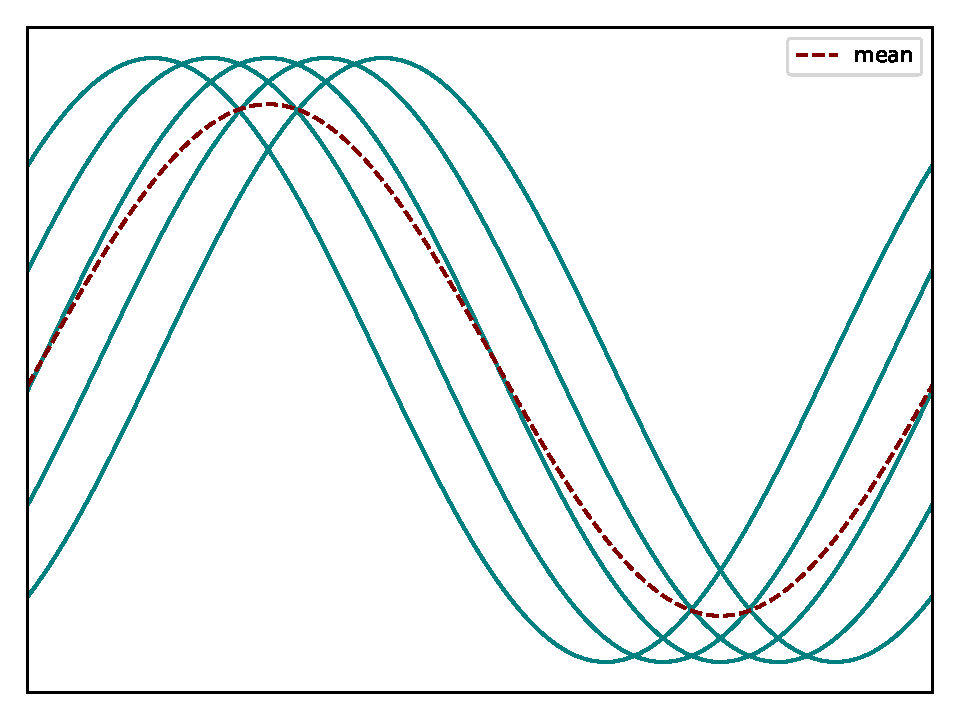
\includegraphics[width=7.5cm]{phase-variation}}
\end{figure}
